\documentclass[UKenglish]{ifimaster}  
\usepackage[utf8]{inputenc}           
\usepackage[T1]{fontenc,url}
\urlstyle{sf}
\usepackage{babel,textcomp,csquotes,duomasterforside,varioref,graphicx}
\usepackage[round]{natbib}

\title{Using Virtual Reality- and Gesture Recognition Technology in Design Reviews}
\subtitle{A Master's Thesis}        
\author{Andreas Oven Aalsaunet}                  

\begin{document}
\duoforside[dept={Department of Informatics},   
  program={Programming and Networks},  
  long]                                        

\frontmatter{}
%% \chapter*{Abstract}                   

\tableofcontents{}
\listoffigures{}
\listoftables{}

\chapter*{Preface}                    
Traditionally the idea of several people interacting in a virtual world, and the emerging virtual reality technologies (e.g Oculus Rift and HTC Vive etc) have been closely tied to the gaming- and entertainment industry. As of this date, these technological advances remains mostly irrelevant for most other industry segments, but could this be about to change? This essay will explore the possibilities of applying these technologies to the design and engineering segment of the industry.

\chapter*{Acknowledgements}  

\mainmatter{}
\part{The state of the field}                   

\chapter{Introduction}                  
The field of virtual- and augmented reality technologies has seen an exciting development in recent years, with the first release of commercial virtual reality devices, such as Oculus Rift and HTC Vive, taking place in 2016. These devices enable the user to be completely emerged in 3D virtual worlds by having one high resolution lens per eye, covering the user's whole field of vision. Although these devices' initial target market was the games- and entertainment industry, the applications of these devices in other domains have already exceeded the expectations of many~\citep{VRS2016}. Examples of such domains include the military, the educational system, the healthcare industry, the construction businesses and the telecommunications industry~\citep{VRS2016}. 

As virtual reality technology enables users to visually perceive virtual worlds in a new way, human-computer interaction (HCI) is also a highly relevant topic. This field has in many ways seen a resurgence as virtual technology gives new possibilities, but also set new constrains. One of these constraints is limiting the user's field of vision exclusively to that projected by the lenses, which may make interaction with traditional input devices, such as mouse and keyboard, more challenging. Because of this, alternate methods of interacting with the computer is a relevant topic. One of these methods is the use of gestures, which have long been considered an interaction technique that can potentially deliver more natural, creative and intuitive methods for communicating with our computers~\citep{Rautaray2015}. 

\section{Outline}
The upcoming master's thesis will explore the possibilities of utilizing virtual reality- and gesture recognition technology in combination during the design review process of the major international classification company DNV GL. This will be accomplished by implementing a design review application that makes use of both these technologies for several design review tasks (see section 2.1), and by having users evaluate the effectiveness of these techniques. This essay will summarize DNV GL's design review process, list the application requirements, discuss some of the developments within the field of gesture recognition technology and briefly review the Leap Motion Controller.


\chapter{Gesture Recognition Technology}
A gesture can be defined as a physical movement of the hands, arms, face and body with the intent to convey information or meaning~\citep{Mitra2007}, and have long been considered an interaction technique that can potentially deliver more natural, creative and intuitive methods for communicating with computers. Even though
the use of keyboard and mouse is a prominent interaction method, there are situations in which
these devices are impractical for human-computer interaction (HCI). This is particularly the case for interaction with 3D objects~\citep{Rautaray2015}. 

To be able to convey semantically meaningful commands through the use of gestures one must rely on a gesture recognition system, which is responsible for capturing and interpreting gestures from the user and, if applicable, carry out the desired action. Often this process is seen as a sum of three fundamental phases: Detection, tracking and recognition~\citep{Rautaray2015}.

\section{Detection}
The first step in a typical gesture recognition system is to detect the relevant parts of the captured image and segment them from the rest. This segmentation is crucial because it isolates the relevant parts of the image from the background to ensure that only the relevant part is processed by the subsequent tracking and recognition stages~\citep{Cote2006}. A gesture recognition system will typically be interested in hand gestures, head- and arm movements and body poses, and thus only these factors should be observed by the system.

\section{Tracking}
The second step in a gesture recognition system is to track the movements of the relevant segments of the frames, e.g.~the hands. Tracking can be described as the frame-to-frame correspondence of the segmented hand regions and aims to understand the observed hand movements. This
is often a difficult task as hands can move very fast and their appearance can change vastly within a few frames, especially when light condition is a big factor~\citep{Wang2010}. One additional note is that if the detection method used is fast enough to operate at image acquisition frame rate, it can also be used for tracking~\citep{Rautaray2015}.   

\section{Recognition}
The last step of a gesture recognition system is to detect when a gesture occurs. This often implies checking against a predefined set of gestures, each entailing a specific action. To detect static gestures (i.e postures involving no movement) a general classifier or template-matcher can be used, but with dynamic gestures (which involves movement) other methods, which keep the temporal aspect, such as a Hidden Markov Model (HMM), are often required~\citep{Benton1995}. The recognition technology often makes uses of several methods from the field of machine learning, including supervised, unsupervised and reinforced learning.

\chapter{Gesture recognition devices}
Creation and implementation of such efficient and
accurate hand gesture recognition systems is aided by two major types of enabling
technologies for human-computer interaction, namely contact-based and vision-based devices~\citep{Rautaray2015}. 

\paragraph{Contact-based devices} are usually wearable objects, such as gloves or armbands, which register the user's kinetic movement through sensors and attempt to mirror it in the virtual world. Some notable products making use of this technology include the Nintendo Wii remote controller and the Myo armband (see figure \ref{fig:myo}). 

\begin{figure}%[h!] %[H]
	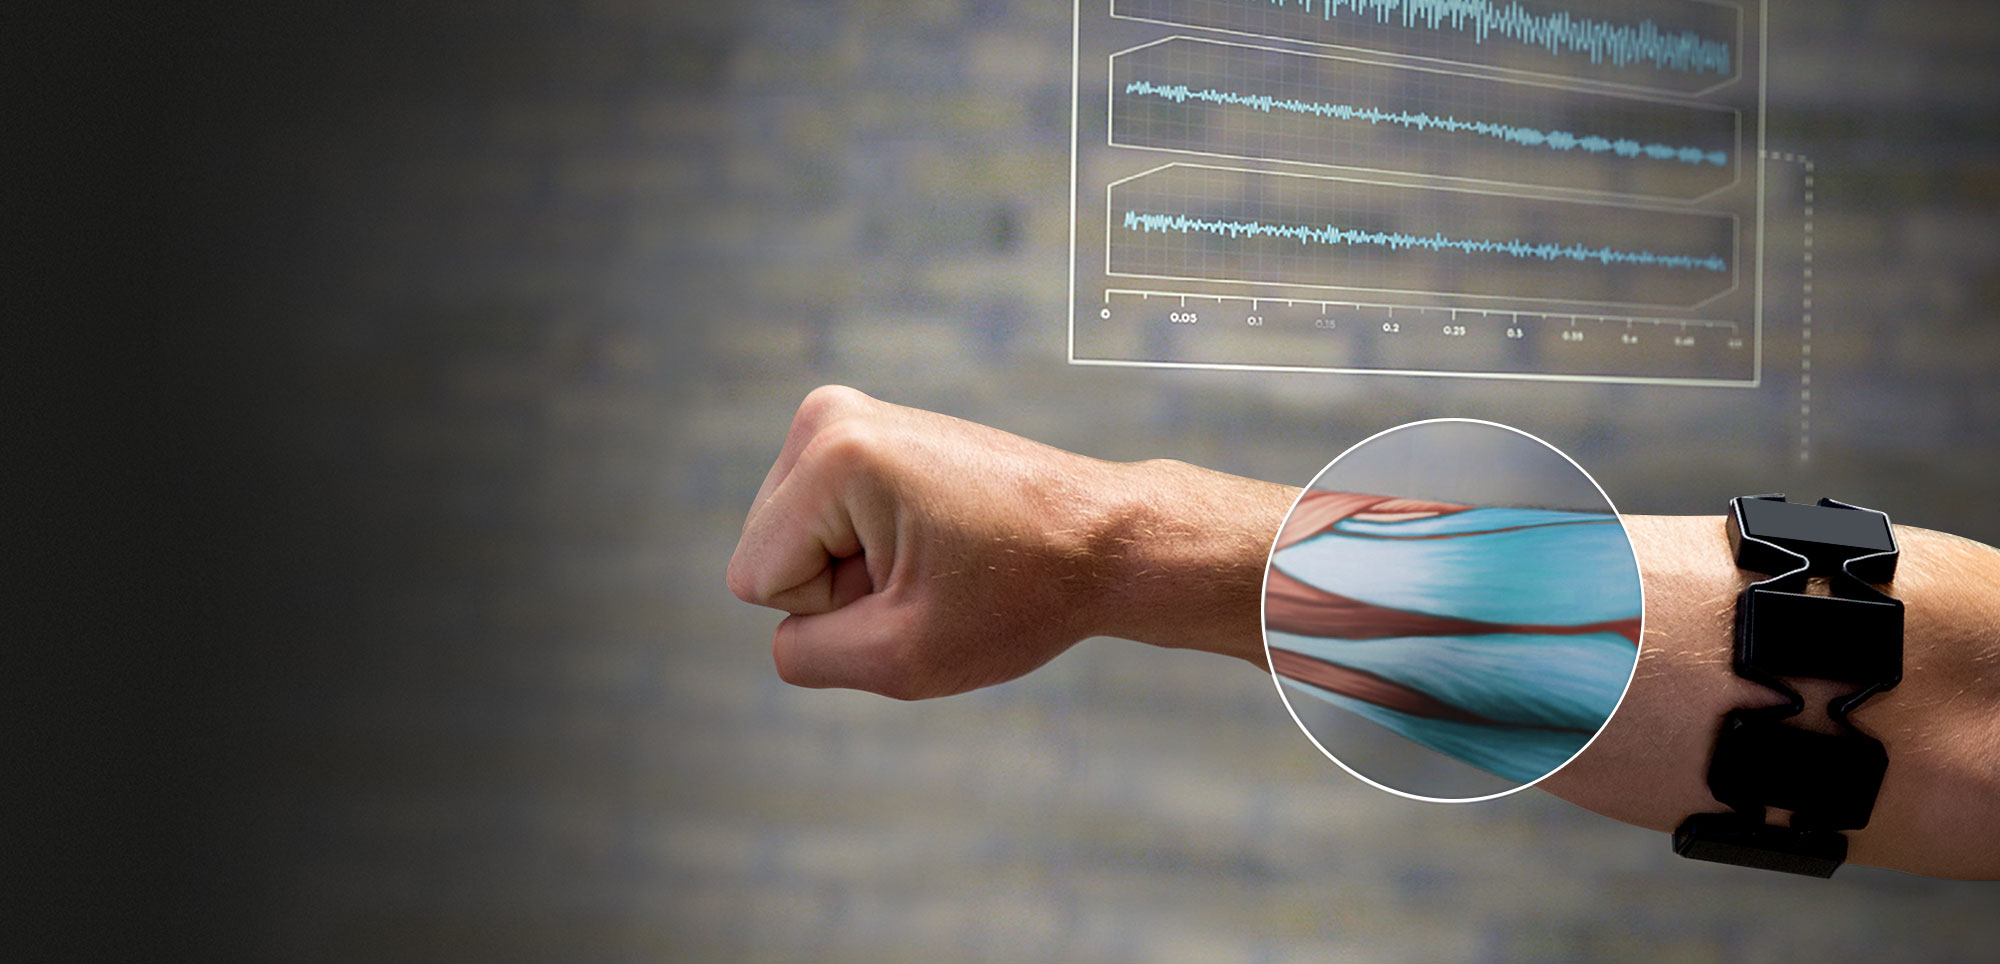
\includegraphics[width=\linewidth]{pictures/myo_armband.jpg}
	\caption{The Myo armband is a gesture recognition device worn on the forearm and manufactured by Thalmic Labs. The Myo enables the user to control technology wirelessly using various hand motions. It uses a set of electromyographic (EMG) sensors that sense electrical activity in the forearm muscles, combined with a gyroscope, accelerometer and magnetometer to recognize gestures~\citep{Myo2015}.}
	\label{fig:myo}
\end{figure}

\paragraph{Vision-based devices} usually make use of either depth-aware cameras or stereo cameras to approximate a 3D representation of what's output by the cameras, which in many ways are similar to how the human eyes work. Products making use of this technology include the Microsoft's Kinect and the Leap Motion controller (see figure \ref{fig:leapmotion}). 

\begin{figure}%[h!] %[H]
	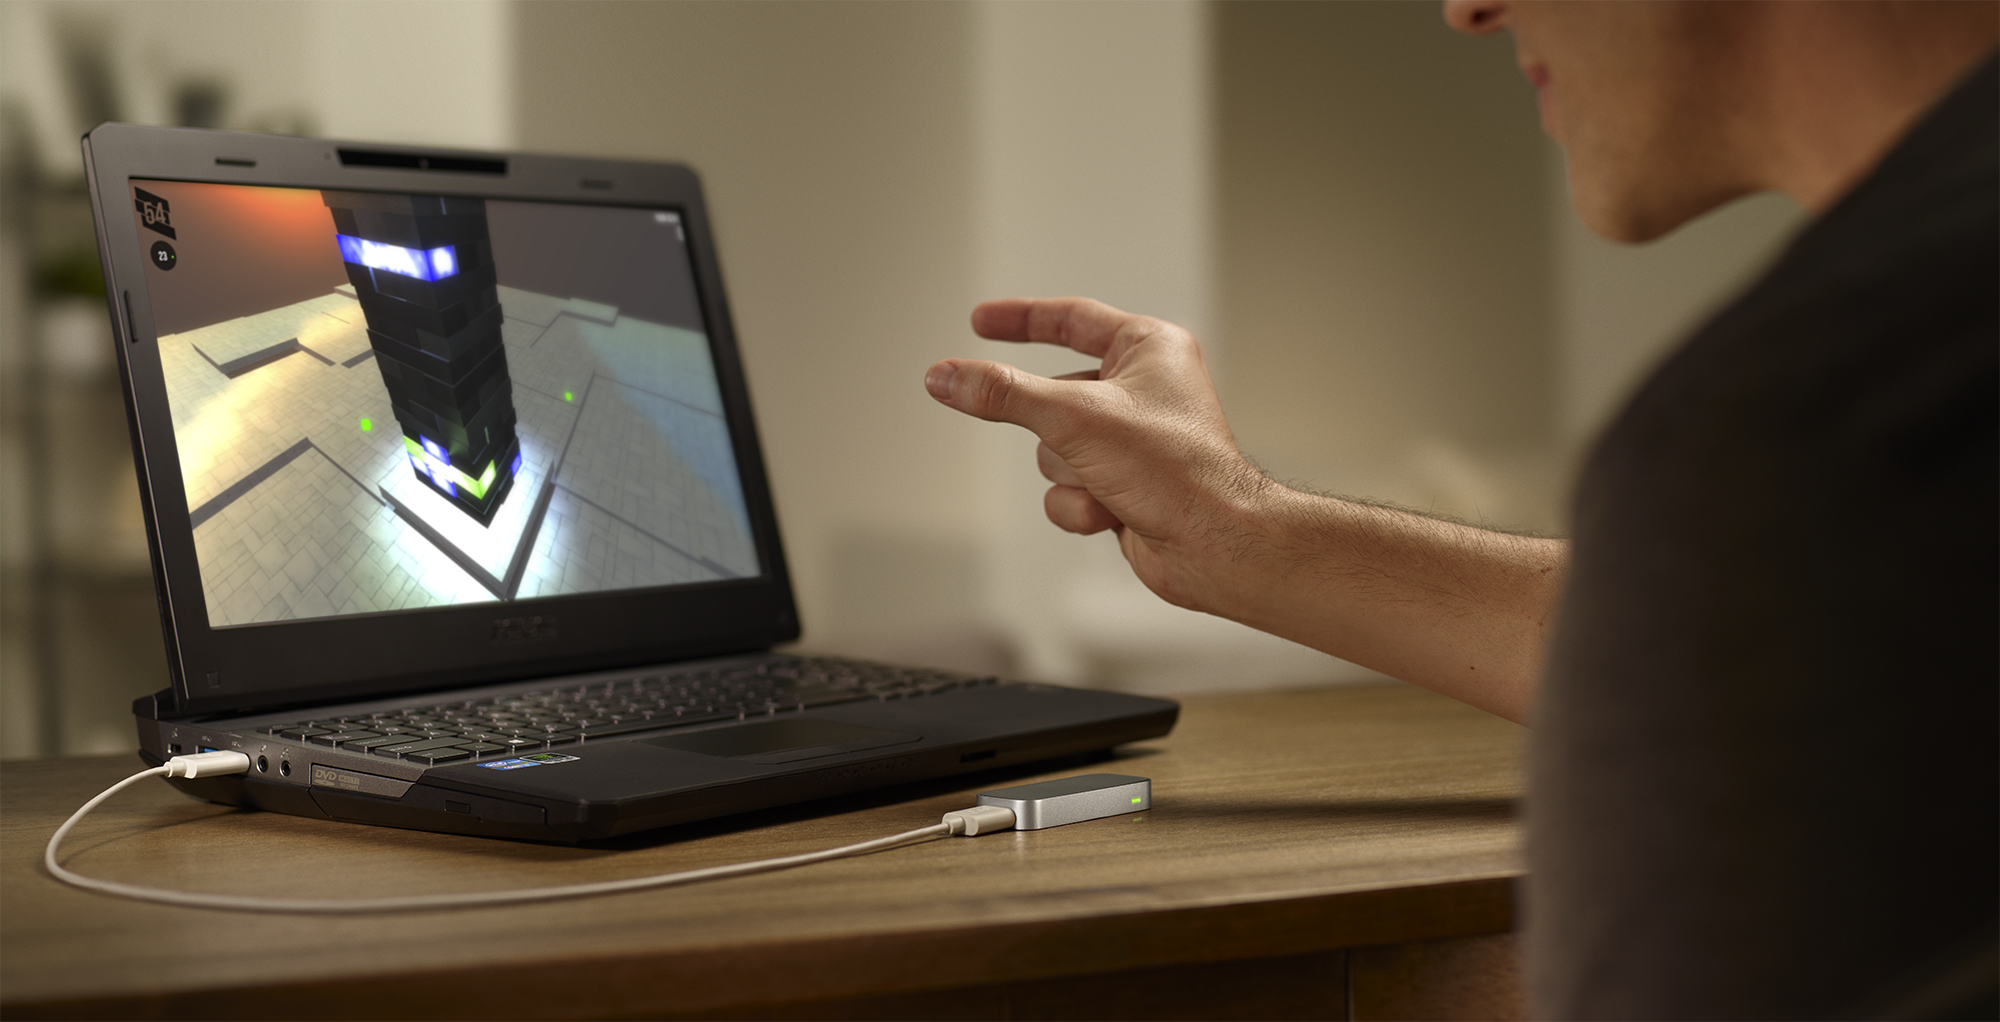
\includegraphics[width=\linewidth]{pictures/leapmotion2.png}
	\caption{The Leap Motion controller is a small USB peripheral device which is designed to be placed on a physical desktop, facing upward. Using two monochromatic IR cameras and three infrared LEDs, the device observes a roughly hemispherical area, to a distance of about 1 meter, and generates almost 200 frames per second of reflected data~\citep{LeapMotion2016}.}
	\label{fig:leapmotion}
\end{figure} 

\paragraph{}Both approaches have their advantages and disadvantages (see~\citet{Rautaray2015} for a deeper discussion of these). Contact-based devices generally have a higher accuracy of recognition and a lower complexity of implementation than that of vision-based ones. Vision-based devices are on the other hand seen as more user friendly as they require no physical contact with the user. 

The main disadvantage of contact-based devices is the potential health hazards, which may be caused by some of its components~\citep{Schultz2003}. Research has suggested that mechanical sensor materials may raise symptoms of allergy and magnetic component may raise the risk of cancer~\citep{Nishikawa2003}. Even though vision-based devices have the initial challenge of complex configuration and implementations, they are still considered more user friendly and hence more suited for usage in long run. Because of the reasons outlined above the master's thesis will primarily be oriented towards vision-based gesture recognition technologies. 

\section{The primary Vision-based Technologies}
Today, there are three primary vision-based technologies that can acquire 3D images: Stereoscopic vision, structured light pattern and time of flight (TOF)~\citep{Ko2012}.
These all make use of one or several cameras and lights to capture and recognize certain movements or poses from the user, and transform it to a certain action on the computer (e.g.~a recognized finger tap might be the equivalent to left mouse button click). 

\paragraph{Stereoscopic vision}is the most common 3D acquisition method and uses two cameras to obtain a left and right stereo image. These images are slightly offset on the same axis as the human eyes. As the computer compares the two images, it develops a disparity image that relates the displacement of objects in the images.

\paragraph{Structured light pattern}measure or scan 3D objects through illumination. Light patterns are created using either a projection of lasers or LED light interference or a series of projected images. By
replacing one of the sensors of a stereoscopic vision system with a light source, structured-light-based technology basically exploits the same triangulation as a stereoscopic system does to acquire the 3D coordinates of the object. Single 2D camera systems with an IR- or RGB-based sensor can be used to measure the displacement of any single stripe of visible or IR light, and then the coordinates can be obtained through software analysis.

\paragraph{Time of flight}is a relatively new technique among depth information systems
and is a type of light detection and ranging (LIDAR) system that transmits a light pulse from an emitter to an object. A receiver determines the distance of the measured object by calculating the travel time of the light pulse from the emitter to the object and back to the receiver in a pixel format.

\begin{figure}%[h!] %[H]
	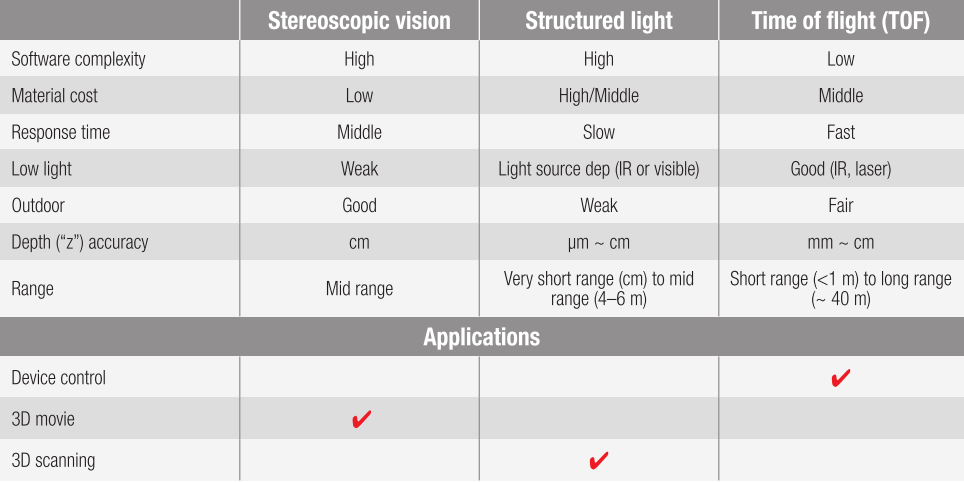
\includegraphics[width=\linewidth]{pictures/Vision-based_comparisons.png}
	\caption{Comparison of Vision-based sensor technologies~\citep{Ko2012}.}
	\label{fig:VBComparisions}
\end{figure} 

\paragraph{Of these technologies} stereoscopic vision is perhaps the most promising one for the consumer market as it has the lowest material cost~\citep{Ko2012}, and has proved more reliable in variable light conditions than its counterparts. One of the latest consumer-oriented devices of this kind is the Leap Motion Controller, which distinguishes itself for having a higher localization precision than other depth vision-based devices~\citep{Weichert2013}, and also for capturing depth data related to palm direction, fingertips positions, palm center position, and other relevant points~\citep{Wei2016}. The Leap Motion Controller will be reviewed more in-depth in the next section. 


\section{How vision-based devices functions}

\chapter{Challenges with VR and GRT} 
Problems with using VR + e.g Leap over mouse + keyboard + display. E.g:

\section{The "writing issue"}
Virtual keyboards are bad. 
Regular keyboards are impractical. 
See "ideer til masteroppgaven.txt"

\section{The VR sickness issue}


\chapter{The Leap Motion Controller}
The latest technological breakthrough in gesture-sensing devices has come in the form of a Leap Motion Controller (Leap Motion, San Francisco, CA, United States). The controller, approximately the size of a box of matches, allows for the precise and fluid tracking of multiple hands, fingers, and small objects in free space with sub-millimeter accuracy~\citep{Guna2014}.

\section{Physical Properties}
The Leap Motion Controller (see fig. \ref{fig:leapmotion} and \ref{fig:leapmotion2}) contains two stereoscopic cameras and three infrared LEDs, which periodically emit a light pulse with a wavelength of 850 nanometer, and thus outside the visible light spectrum. During the light pulses, which light up about eight cubic feet in front of the controller, grayscale stereo images are captured by the cameras and sent to the Leap Motion tracking software~\citep{LeapMotion2016}. In the software, the images are analysed to reconstruct a 3D representation of what the device sees, compensating for static background objects and ambient environmental lighting. 

\begin{figure}%[h!] %[H]
	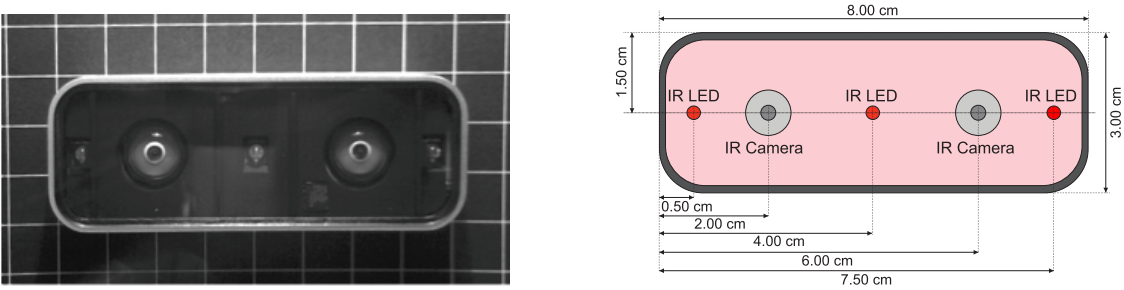
\includegraphics[width=\linewidth]{pictures/LMC_measures.png}
	\caption{Visualization of a Leap Motion Controller, with Infrared Imaging (left) and a Schematic View (right)~\citep{Weichert2013}.}
	\label{fig:leapmotion2}
\end{figure} 

\section{The Leap API}
The controller itself can be accessed and programmed through Application Programming Interfaces (APIs), with support for a variety of programming languages, including C++, C\#, Objective-C, Java, JavaScript and Python. Although the API is programmed almost exclusively in C, access through a variety of other languages is achieved by virtue of various "wrapper libraries", which exposes and translates functions from their respective languages into the corresponding C function[cite].

The Leap Motion SDK also features integration with commercial game engines such as Unity and the Unreal Engine~\citep{Guna2014}. One example of what the Leap Motion API enables is acquisition of the recognized object's position through Cartesian and spherical coordinate systems, which are used to describe positions in the controller's sensory space~\citep{Guna2014}.  

Technically, very few details are publicly known about the precise nature of the algorithms used due to patent and trade secret restrictions.

\subsection{Important Leap components}
Hands, fingers, palm, directions, frames, interaction box etc. See 
https://developer.leapmotion.com/documentation/csharp/devguide/Leap\_Overview.html\#motion-tracking-data
https://developer.leapmotion.com/documentation/csharp/devguide/Leap\_Coordinate\_Mapping.html\#map3d
https://developer.leapmotion.com/documentation/csharp/devguide/Leap\_Hand.html


\subsection{Detectors - The building blocks of gesture recognition}
The detector scripts. How they can be combined. Logic gates. 
See https://developer.leapmotion.com/documentation/unity/unity/Unity\_DetectionUtilities.html

\subsection{Integration with the Unity editor}
How the pieced fit together. How the stuff is organized (e.g the modules).
See https://developer.leapmotion.com/documentation/unity/index.html


\part{The project} 

\chapter{Background and motivation}

\section{The resurgence of virtual reality technology}

\section{DNV GL and their motivations}
DNV GL is the world's largest classification society with more than 13 000 vessels and mobile offshore units, which represents a global market share of 21\%~\citep{TO:DNVGL}. It is the world's largest technical consultancy to onshore and offshore wind, wave, tidal, and solar industries, as well as the global oil \& gas industry -- 65\% of the world’s offshore pipelines are designed and installed to DNV GL technical standards~\citep{MTN:DNVGL}. A major part of DNV GL's work is evaluation and quality assurance of a client's product (e.g.~a ship) , where a DNV GL "Approval Engineer" conducts a design review of the client's model of the proposed product. This process usually consists of the following steps: 

\begin{enumerate}
	\item The designer sends the model to DNV GL for evaluation.
	\item The approval engineer inspects the model noting down aspects that doesn't meet DNV GL requirements.
	\item The designer receives the remarks and makes the necessary changes to the model.
	\item This process is repeated until both parties are satisfied.
\end{enumerate}

DNV GL is looking into the possibilities of making this process more interactive, effective and simultaneous using virtual reality- and gesture technologies to conduct virtual design review meetings in the 3D models. The idea is to create sessions that enable both parties to be virtually present in the same instance of the 3D model, and to interact with it. The parties present should be able to navigate the 3D model, annotate problems, link the problems to predefined rules or requirements and see representations of each other (i.e through a character model/avatar). The application should also support a model versioning system to keep track of which model version(s) annotations are tied to.

At the end of a session the 3D model may contain one or several annotations, which the designer then has to address before the design can be approved. A more detailed list of application demands is described below.

\section{Application requirements}
This section gives an overview of the desired use cases for the finished application. When the user
wishes to initiate or join a session with a particular 3D model to be inspected, he/she should be able to:
\begin{itemize}
	\item Choose between hosting or joining a session.
	\item If the user wishes to host a session, he/she should be able to specify a 3D model from a standard file format (such as FBX files).
	\item If the user wishes to join a session, he/she should be able to choose an open session from a list of available sessions.
\end{itemize}
Once a user has either created or joined a session and is loaded into the model, he/she should be able to:
\begin{itemize}
	\item Look around, e.g.~by using mouse movements or head motions (picked up from sensors in the VR head device).
	\item Move around on the horizontal plane by using the arrow keys, the WASD keys or by specific gestures (e.g.~a "dragging motion").
	\item Move in the vertical plane increasing or decreasing altitude (i.e "flying").
	\item Zoom in and out by virtually changing the avatar's own size.
	\item Annotate the surface he/she is looking at. This should furthermore enable:
	\begin{itemize}
		\item Choosing between a placeholder-, predefined- or custom defined text and/or an icon.
		\item Choosing between several annotation states,  e.g.~"unresolved", "work in progress", "Ready for approval" and "approved".
		\item Automatic saving of the annotation and its coordinates to a log used for easy retrieval of the annotation entries. 
		\item A threaded follow up discussion of the annotation (i.e adding comments).
	\end{itemize}
	\item Annotate regions or areas of the 3D model (e.g.~annotate an entire room). These "area annotations" should subsequently be modifiable to change the size. 
	\item Link annotations to the DNV GL rules and requirements.
	\item Draw on the desired surface to make suggestions or highlight, e.g.~drawing arrows.
	\item Choose between enabling or disabling collision and gravity. By default the user should be able to traverse freely without collision, but to enable it can be practical in certain circumstances.
	%\item Make the target surface transparent and without collision, thereby enabling the user to %move through it.
	\item Obtain the real-world distance between two specified points.
	\item Bookmark the avatar's current location and orientation to easily be able to go back to bookmarked locations. 
\end{itemize}

Actions done during the 3D model session (such as annotating an object) should continuously be stored in a database. If a user wants to re-enter the session at a later time, this database is read, and the actions done in previous sessions are loaded into the model. By utilizing a database 
in this way the model files themselves can also remain unedited throughout a session, as opposed to saving annotations into the model files itself, which could be more inefficient and create model versioning issues. Another upside with utilizing a database is that it enables exposure of the actions done in the sessions to other platforms, such as web applications. This can enable annotation and comments done on the 3D model to become "issues" or "remarks" in more traditional collaboration tools such as Atlassian's Jira or Confluence, although this will not be a focus point for the thesis.  

To ensure that the desired application is as intuitive and functional as possible the upcoming master's thesis will also look into several ways of interacting with the 3D model while using virtual reality lenses. Special emphasis will be put on using gestures for certain tasks (such as marking and annotating objects) and evaluating the performance through user testing. Using gestures in combination with mouse and keyboard, game controller and joysticks will also be evaluated to ensure a satisfactory user experience.     

\chapter{Review of the implementation}

\section{The gestures}
\subsection{Challenges in "designing" gesture schemes}
People have different preferences. Have intuitive gestures. Have gestures that is not too
fatiguing. Have gesture with high precision and recall (F-score) (high TP and TN. Low FP, FN).
Have a system that doesnt mistake one gesture for another.

\subsubsection{Fixes?}
User-gesture calibration. 

\subsection{The pinch gesture}
\subsection{The straight-hand gesture}
\subsection{The fist gesture}
\subsection{The point gesture}

\chapter{The user testing sessions}




\chapter{Conclusion}
This essay has given a brief summary of the virtual reality design review application that is going to be implemented for DNV GL as part of the master's thesis, and how virtual reality- and gesture recognition technology can be utilized to potentially improve the human-computer interaction experience beyond that of more conventional interaction methods. 

Gesture recognition technology is often divided into the categories of vision-based and contact-based, where the former usually is the preferred one because of user-friendliness and the health concerns associated with the latter. Vision-based gesture recognition devices usually utilize either stereoscopic vision-, structured light pattern- or time of flight techniques, where stereoscopic vision-based devices have proved the most promising. One device of this kind is the Leap Motion Controller, which consists of two stereoscopic cameras and three infrared LEDs and periodically captures grayscale stereo images which are sent to the tracking software, where 3D representations are constructed. 

The master's thesis aims to evaluate the performance and user experience of utilizing a Leap Motion Controller in combination with the Oculus Rift and HTC Vive virtual reality headsets during a virtual design review in a complex 3D model. The final application should thus be primarily focused on utilizing the most intuitive ways of interacting with complex 3D models in a collaborative virtual reality setting.     	                                     

%Through previous research endeavours vision-based gesture recognition devices has proved to be the most promising ones, and it has already seen some moderate commercial success through devices such as the XBox Kinect and the Leap Motion Controller. However, many previous research articles states that the techniques implemented for hand gesture recognition often are sensitive to poor resolution, frame rate, drastic illumination conditions, changing weather conditions and occlusions among other prevalent problems in the hand gesture recognition systems~\citep{Rautaray2015}.

%Despite these reported shortcomings, the upcoming master's thesis will explore areas where gesture recognition technology might perform in a sufficient manner, and also explore how a gesture recognition system can be used in combination with more traditional input-methods, such as a mouse, keyboard, gamepad or joystick. The final application implementation should thus be primarily focused on utilizing the most intuitive ways of interacting with complex 3D models in a virtual reality setting.   

%the use cases for these are still somewhat limited and has often been reported to not have a reliable enough tracking and recognition~\citep{Guna2014}. 

\backmatter{}
\bibliography{references}
\bibliographystyle{apalike}
\end{document}
